\documentclass[11pt,
  paper=a4, 
  bibliography=totocnumbered,
	captions=tableheading,
	BCOR=10mm
]{scrreprt}

\usepackage[utf8]{inputenc}
 
 
\usepackage[onehalfspacing]{setspace}
\usepackage{csquotes} % Context sensitive quotation.
\usepackage{amsmath} % Standard math.
\usepackage{amsthm} % Math theorems.
\usepackage{amssymb} % More math symbols.
\theoremstyle{definition}
\newtheorem{definition}{Definition}[chapter]
 
\usepackage[section]{placeins} % Keep floats in the section they were defined in.
\usepackage{tabularx}
\usepackage{booktabs} % Scientific table styling.
\usepackage{floatrow} % Option for keeping floats in the place they were defined in the code.
\floatsetup[table]{style=plaintop}
\usepackage{hyperref} % Hyperlinks.
\usepackage[all]{nowidow} % Prevent widows and orphans.
\usepackage{xstring} % logic string operations
\usepackage[nopostdot, nonumberlist]{glossaries} % glossary for definitions and acronyms, without dot after entry and page reference 
\usepackage{bbm} % \mathbb on numerals.
\usepackage{csquotes}
\usepackage{mathtools}
\usepackage[ruled,vlined]{algorithm2e} %Pseudocode
\usepackage{scrhack} % Make warning go away.
\usepackage{graphicx}
\usepackage{subcaption} % Subfigures with subcaptions.
\usepackage{authoraftertitle} % Make author, etc., available after \maketitle
\usepackage{listofitems}
\usepackage{blindtext} % Placeholder text.
\usepackage[nopostdot, nonumberlist]{glossaries}
\usepackage{soul}
\makeglossaries % Generate the glossary

% \PassOptionsToPackage{obeyspaces}{url}%
\usepackage[backend=bibtex,% 
style=nature,% 
doi=true,isbn=false,url=false, eprint=false]{biblatex}
% \renewbibmacro*{url}{\printfield{urlraw}}

\addbibresource{bib/library.bib}

\DeclareStyleSourcemap{
  \maps[datatype=bibtex, overwrite=true]{
    \map{
      \step[fieldsource=url, final]
      \step[typesource=misc, typetarget=online]
    }
    \map{
      \step[typesource=misc, typetarget=patent, final]
      \step[fieldsource=institution, final]
      \step[fieldset=holder, origfieldval]
    }
  }
}

%\linespread{1.5} % set line spacing
 
\usepackage{listings} % rendering program code
\lstset{% general command to set parameter(s)
	basicstyle=\ttfamily\color{grey},          % print whole listing small
	keywordstyle=\color{black}\bfseries\underbar,
	% underlined bold black keywords
	identifierstyle=,           % nothing happens
	commentstyle=\color{white}, % white comments
	stringstyle=\ttfamily,      % typewriter type for strings
	showstringspaces=false}     % no special string spaces


\DeclareFontFamily{U}{mathx}{\hyphenchar\font45}
\DeclareFontShape{U}{mathx}{m}{n}{
      <5> <6> <7> <8> <9> <10>
      <10.95> <12> <14.4> <17.28> <20.74> <24.88>
      mathx10
      }{}
\DeclareSymbolFont{mathx}{U}{mathx}{m}{n}
\DeclareFontSubstitution{U}{mathx}{m}{n}
\DeclareMathSymbol{\bigtimes}{1}{mathx}{"91}

 

%%% Custom definitions %%%
% Shorthands
\newcommand{\ie}{i.\,e.~}
\newcommand{\eg}{e.\,g.~}
\newcommand{\ind}{\mathbbm{1}}
% Functions
\newcommand{\tpow}[1]{\cdot 10^{#1}}
\newcommand{\figref}[1]{(Figure \ref{#1})}
\newcommand{\figureref}[1]{Figure \ref{#1}}
\newcommand{\tabref}[1]{(Table \ref{#1})}
\newcommand{\tableref}[1]{Table \ref{#1}}
\newcommand{\secref}[1]{%
	\IfBeginWith{#1}{chap:}{%
		(cf. Chapter \ref{#1})}%
		{(cf. Section \ref{#1})}%
		}
\newcommand{\sectionref}[1]{%
	\IfBeginWith{#1}{chap:}{%
		Chapter \ref{#1}}%
		{\IfBeginWith{#1}{s}{%
			Section \ref{#1}}%
			{[\PackageError{sectionref}{Undefined option to sectionref: #1}{}]}}}
\newcommand{\chapref}[1]{(see chapter \ref{#1})}
\newcommand{\unit}[1]{\,\mathrm{#1}}
\newcommand{\unitfrac}[2]{\,\mathrm{\frac{#1}{#2}}}
\newcommand{\codeil}[1]{\lstinline{#1}}{} % wrapper for preventing syntax highlight error
\newcommand{\techil}[1]{\texttt{#1}}
\newcommand{\Set}[2]{%
  \{\, #1 \mid #2 \, \}%
}
% Line for signature.
\newcommand{\namesigdate}[1][5cm]{%
	\vspace{5cm}
	{\setlength{\parindent}{0cm}
	\begin{minipage}{0.3\textwidth}
		\hrule 
		\vspace{0.5cm}
		{\small city, date}
	\end{minipage}
	 \hfill
	\begin{minipage}{0.3\textwidth}
		\hrule
		\vspace{0.5cm}
	    {\small signature}
	\end{minipage}
	}
}
% Automatically use the first sentence in a caption as the short caption.
\newcommand\slcaption[1]{\setsepchar{.}\readlist*\pdots{#1}\caption[{\pdots[1].}]{#1}}

% Variables. 
% Adapt if necessary, use to refer to figures and graphics.
\def \figwidth {0.9\linewidth}
\graphicspath{ {./graphics/figures/}{./graphics/figures/} } % Path to figures and images.


% Customizations of existing commands.
\renewcommand{\vec}[1]{\mathbf{#1}}
% Capitalized \autoref names.
\renewcommand*{\chapterautorefname}{Chapter}
\renewcommand*{\sectionautorefname}{Section}


% TODO Fill with your data.
\title{On the potential of recurrent structures for semantic video segmentation with deep networks}
\author{Sven Groen}

\begin{document}

\begin{titlepage}
	\begin{flushleft}
		Universität Osnabrück\\
		Fachbereich Humanwissenschaften\\
		Institute of Cognitive Science
	\end{flushleft}

	\vspace{2cm}
	\centering{
		Bachelorthesis - Expose \vspace{1cm}\\
		\textbf{\Large{\MyTitle}}
		\vspace{1cm}\\
		\begin{tabular}{c}
			\MyAuthor                          \\
			970219                            \\
			Bachelor's Program Cognitive Science 
		\end{tabular}}
	\vspace{1cm}

	\begin{tabular}{ll}
		First supervisor:  & Dr. Ulf Krumnack          \\
		                   & Institute of Cognitive Science            \\
		                   & Osnabrück                \\\\
		Second supervisor: & Manuel Kolmet         \\
		                   & IMANOX GmbH  \\
		                   & Berlin 
	\end{tabular}

\end{titlepage}


\pagenumbering{gobble}
\pagebreak


\tableofcontents


\chapter{Goal and background information}
\pagenumbering{arabic}

\section{Cooperation with IMANOX}
This project is realized in cooperation with \href{https://www.Imanox.de/}{IMANOX}. 
IMANOX is a Berlin-based startup that developed a smart photo booth for expositions, events and promotions. 
The photo booth enables customers virtual product placements using augmented and mixed reality. 
Main features are hand-tracking, digital masks and changing virtual backgrounds.

\section{Virtual backgrounds}
Currently, the photo booth developed by IMANOX is using a built in Kinect RGB-D camera that measures the distance of objects by casting infrared illumination onto the scene and indirectly measuring the time it takes to travel back to the camera. 
The camera struggles with correctly predicting the depth in certain situations. 
Pixels are rendered as invalid and no depth information is provided. 
The reasons for this are numerous. 
Pixels might get undersaturated (signal is not strong enough) or oversaturated (signal is too strong). 
Other artifacts occur due to the geometry of the scene. 
For example, the sensors of the camera might receive signals from multiple locations in the scene, leading to an ambiguous depth. 
Especially around the edges and borders of objects pixels contain mixed signals from fore- and background, leading to blurred outlines.
In the current version of the photo booth, alpha values (0 to 1) are calculated based on the data from the depth sensor. 
This is done by applying an alpha matting algorithm \cite{Gastal2010} to the raw depth data.
Objects in the foreground receive high alpha values and the background is considered to have an alpha value of 0, making it transparent. 
In this way, the background can be virtually replaced without affecting the objects in the foreground. 
Due to the described inaccurate data that is given by the depth sensor, the result is of low quality. 
The edges and borders of the objects or people in the scene are not sharp and often misclassified. 
Especially for small and thin objects like hair, the camera hardly recognizes them and parts of the objects are therefore misclassified as background and are also replaced by the virtual background.
For more detailed information on this issue see \url{https://docs.microsoft.com/de-de/azure/Kinect-dk/depth-camera} \cite{Microsoft2019}.

\section{Goal of the thesis}
The goal of this bachelor thesis is to improve the quality of the semantic segmentation of the current IMANOX photo booth using machine learning techniques.
The machine learning model will be one of the artificial neural network architectures (see Section~\ref{sec:related_work} for details).
This model will be altered and changed towards the needs of the project and will be trained with custom training data.
It will be investigated whether additional temporal information leads to an improvement of the already existing segmentation models (see Section~\ref{sec:Method}).
When looking at succesful semantic segmentation models, it can be noticed that the prediction occurs on bases of individual images.
It can be argued that in \textit{real world scenarios} a semantic segmentation on single images is not as required as it is on videos, which are streams of frames.
Potential applications include autonomous driving or video effects in the film industry.


When working with video data, valuable temporal information might get lost when the segmentation occurs on individual frame level.
Therefore, the thesis will investigate whether the temporal information that is present in video data can be used for improvement of performance by adding recurrent structures
into existing semantic segmentation models. 
Given the collaboration with IMANOX and their goal to replace their \textit{virtual background change}-technique, the focus of the thesis will be on binary semantic segmentation
instead of the typical multiclass segmentation. 


\chapter{Segmentation of Images}
\textcite{Szeliski2011} refers to image segmentation as "the task of finding groups of pixels that 'go together'" (\cite{Szeliski2011}, p. 237).
How the pixels are \textit{grouped together} can be achieved in different ways.
In the classical image classification tasks, the task is to simply name the objects that can be seen in an image.
Semantic image segmentation extends this problem further, referring to a pixel-wise classification of an image \cite{Minaee2020}.
Each pixel in an image is assigned to one category label given a set of categories.
However, individual instances of an object in one image are not differentiated but labeled as one class.
Instance segmentation combines a pixel-wise classification (similar to semantic segmentation) with an additional object detection and localization, differentiating each individual instance of a class \cite{Minaee2020}.
Given the goal of this project, only binary semantic segmentation is necessary.
Detailed information about which objects are in the scene is not required.
\begin{figure}[H]
	\centering
	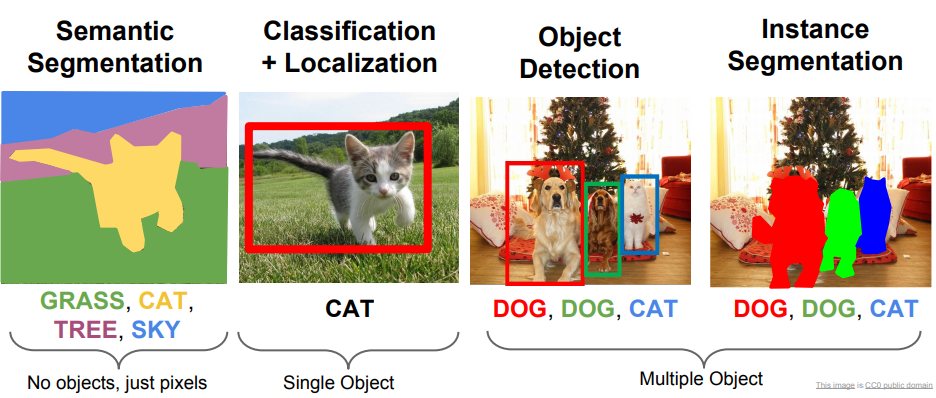
\includegraphics[width=\figwidth]{Computer_Vision_Tasks}
	\slcaption{
		Overview of Computer Vision Tasks. (\textcite{Fei-Fei2017}, Slide 17).
		\label{fig:Computer_Vision_Tasks}}
\end{figure}

\section{Related work}
\label{sec:related_work}

Segmenting an image into its individual parts is a classical problem of computer vision \cite{Szeliski2011}. 
Early approaches involve typical methods like threshold detection \cite{Smith1979}.
More modern approaches like k-means clustering \cite{Dhanachandra2015} improved the early results.
Deep learning architectures, especially convolutional neural networks (CNNs) \cite{Fukushima1980}, have lead to further improvement.
\textcite{Shelhamer2017} have been the first to propose a CNN architecture where a pixel-wise supervised training was achieved. 
This was done by upsampling the class prediction layer to the input image size, leading to an end to end pixel-wise classification, a \textit{Fully Convolutional Network} (FCN) \cite{Shelhamer2017}.
Following papers proposed different architectures.
A \textit{Deconvolutional Network} with special unpooling and deconvolution operations was invented by \textcite{Noh2015}. 
Here, the information was enconded using several convolutions and poolings and was decoded using unpooling and deconvolution.
The SegNet model uses a similar Encoder-Decoder architecture by using pooling indices to upsample the image \cite{Badrinarayanan2017}.
ICNet \cite{Zhao2017} was able to perform semantic segmentation not only in real-time, but also for high quality images (1024x2048 at 30 fps). 
This was achieved by using a cascade image input of different resolutions. 
The authors made use of the semantic information from the scaled down images and the details from the high resolution images.
In this way, they have been able to achieve a "trade-off between efficiency and accuracy" (\cite{Zhao2017}, p.2).
Google's approach towards instance segmentation is called Deeplab and has evolved over the last recent years.
The first DeepLab version uses a combination of Deep CNNs with fully connected conditional random fields (CRFs) that tries to grasp the semantic context of the image \cite{Chen2018}. 
One of their main contributions is the use of atrous (or dilated) convolutions as an alternative to deconvolution. 
Originally used for wavelet transformations, a new parameter r allows to change the stride at which the samples are taken during the convolution operation \cite{Chen2018}.
This approach has been further improved and Atrous Spatial Pyramid Pooling (ASPP) \figref{fig:ASPP} has been introduced, which was based on the idea of combining atrous convolutions with spatial pyramid pooling \cite{Chen2018a} (firstly introduced by \textcite{He2014}).
In ASPP, parallel filters of different dilation rates are concatinated with the intend to cover different field-of-views \cite{Chen2018a}.
The most recent approach, DeepLab V3+, has an Encoder-Decoder structure and was able to show "new state-of-the-art performance on PASCAL VOC 2012 and Cityscapes datasets." (\cite{Chen2018b}, p.14).
Moreover, the Google research team has shown that they are able to create an Encoder-Decoder architecture that is very light and fast.
This architecture is light enough to run at real-time on modern smartphones \cite{Bazarevsky2018}.


\begin{figure}[H]
	\centering
	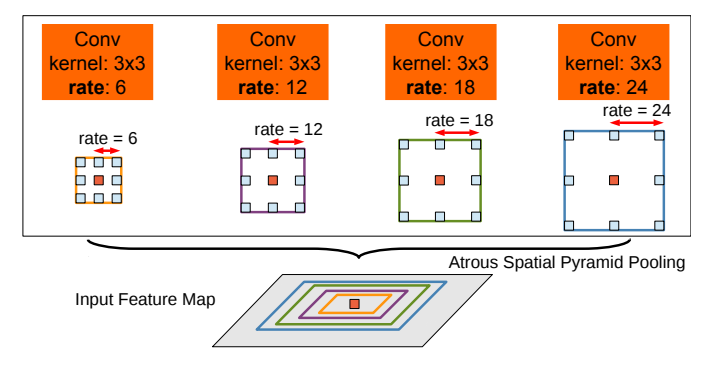
\includegraphics[width=\figwidth]{ASPP}
	\slcaption{
		Atrous Spatial Pyramid Pooling. (\cite{Chen2018a}, Fig. 4).
		\label{fig:ASPP}}
\end{figure}


Most of the models are usually evaluated on individual images.
However, in real world scenarios segmentation is often necessary for videos and not just single images.
Naturally, the segmentation works on each individual frame but the context of the videos gets lost.
The model is not able to know that the previous frame is related to the current one, it treats each frame independently.
Extending existing models with a recurrent unit could enable the model to not only use spatial but also spatiotemporal information.
Recurrent neural networks (RNNs), a special kind artificial neural networks, are usually the answer to time dependent problems \cite{Hoffmann2017} or used for sequential data such as in time series analysis or text translation.
They are known to suffer from the \textit{vanishing- and exploding-gradient-effect} \cite{Sherstinsky2020}.
To account for this problem, Long-Short-Term-Memory cells have been invented by Hochreiter and Schmidhuber \cite{Hochreiter1997} introducing a set of gates that enable the model to selectively forget, learn or keep specific information.
Gated Recurrent Networks (GRUs) work in a similar way while being more efficient since less gates are available \cite{Chung2014}.
Research has been shown (\eg \cite{Nabavi2018, Pfeuffer2019, Pfeuffer2_2019}) that using Convolutional Long-Short-Term-Memory ("Conv-LSTM" \cite{Shi2015}) layers help to improve the performance of already existing architectures.
However, introducing a recurrent unit comes with the downside of increased computational complexity \cite{Pfeuffer2_2019}.


\section{Challenges}

There are several problems that have to be considered during the project:
\begin{enumerate}
	\item achieving invariance towards environmental changes (moving, occluding/overlapping objects)
	\item achieving a good trade-off between high-quality results and low-inference time 
	\item sucessfully integrating recurrent units (conv-LSTMs and conv-GRUs) into an already existing architecture
\end{enumerate}

In order to achieve the first challenge the recurrent units in form of LSTM and GRU cells will be integrated.
The assumption here is that this enables the model to recognize how the objects move throughout time and learn how to cope with uncertainty in situations where objects occlude each other.
\textcite{Pfeuffer2019, Pfeuffer2_2019} have already shown that adding LSTMs has a massive influence on the number of parameters and inference time of the model.
Therefore, the thesis will investigate whether the potential performance increase justifies the increased complexity (second challenge).
For this reason, it is important to carefully consider where and how the recurrent units could be integrated in the model (third challenge).


\chapter{Method}
\label{sec:Method}

Since the main task is to separate humans (and objects they might carry) from the background, training data will be generated using green screen footage.
A green screen setup allows to separate the background in a high quality manner using an alpha matting algorithm (\eg \cite{Gastal2010}).
The background in the training data can be virtually replaced with backgrounds that will be used in the photo booth in the final product.

It is very likely that the model will not be able to generalize very well beyond the given backgrounds, since the training data environment is highly controlled and fixed.
Usual steps to cope with overfitting, \eg data augmenting, will be explored during the training.
However, the final model does not have to generalize beyond the given scenario anyway. 

The project will use the most recent DeepLab architecture (DeepLabV3+) with different backbones.
It will be investigated whether the complexity of the backbone has an influence on the performance change.
Conv-LSTM and Conv-GRU cells will be integrated to the base models.
The base model will be compared with their LSTM/GRU counterpart.

Depending on the time and scope that is left after the major questions have been evaluated, additional aspects will be explored.
These include testing the model on a different dataset (probably Cityscapes dataset) and testing different models besides the DeepLabV3.



\chapter{Preliminary structure}

\begin{itemize}
	\item Declaration of Authorship
	\item Abstract
	\item Contents
	\item List of figures
	\item List of algorithms
	\item Introduction
	\begin{itemize}
		\item Motivation
		\item Goal of the thesis
		\item Semantic Segmentation
		\item Recurrent Neural Networks
		\item Related work
	\end{itemize}
	\item Methods
	\begin{itemize}
		\item The Dataset
		\item Preprocessing
		\item Network architecture
		\item Network training
	\end{itemize}
	\item Results 
	\item Evaluation and discussion
	\item Conclusion
	\item Acknowledgements
	\item Bibliography
\end{itemize}

\chapter{Time frame}

\begin{table}[h]
	\begin{tabular}{|l|l|l|}
	\hline
	\textbf{Week} & \textbf{Date}           & \textbf{What will be done}                                                                                                          \\ \hline
	1-2  		  & \st{01.04.2020 - 14.04.2020} & \begin{tabular}[c]{@{}l@{}}\st{fixing the topics that will be investigated,} \\ \st{fixing the model that will be used} \end{tabular} \\ \hline
	2-4  		  & \st{15.04.2020 - 28.04.2020} & \begin{tabular}[c]{@{}l@{}}\st{preparing and recording training data,} \\ \st{preprocess training data}\end{tabular}                 \\ \hline
	4-8  		  & \st{29.04.2020 - 26.05.2020} & \begin{tabular}[c]{@{}l@{}}training the model, \\ evaluating and analysing the results, \\ start writing\end{tabular}      \\ \hline
	8-12 	 	  & 27.05.2020 - 22.06.2020 & \begin{tabular}[c]{@{}l@{}}fix potential issues, \\ finish implementation, \\ finish writing,\end{tabular}                 \\ \hline
	12   		  & 23.06.2020              & finish thesis                                                                                                              \\ \hline
	\end{tabular}
	\slcaption{
		Previous time frame
		\label{time_frame}}
\end{table}

\begin{table}[h]
	\begin{tabular}{|l|l|l|}
	\hline
	\textbf{Week} & \textbf{Date}           & \textbf{What will be done}                                                                                                          \\ \hline
	1-4  		  & 01.06.2020 - 01.07.2020 & \begin{tabular}[c]{@{}l@{}}finish integration of LSTM/GRU into DeepLab \\ finish "Introduction" \end{tabular} \\ \hline
	4-8  		  & 02.07.2020 - 31.07.2020 & \begin{tabular}[c]{@{}l@{}}finish training and evaluation \\ end writing of thesis \end{tabular}                 \\ \hline
	8-12 	 	  & 01.08.2020 - 30.08.2020 & \begin{tabular}[c]{@{}l@{}}proofreading \\ (extend evaluation by additional models/datasets)\end{tabular}                 \\ \hline
	12   		  & 30.08.2020              & finish thesis                                                                                                              \\ \hline
	\end{tabular}
	\slcaption{
		Updated time frame
		\label{time_frame}}
\end{table}
% Acronym definitions
%TODO Add acronym definitions produced by acronyms2glossary.py 




\glsaddall
\printglossaries

\printbibliography

\end{document}